\documentclass[
  shownotes,
  xcolor={svgnames},
  hyperref={colorlinks,citecolor=DarkBlue,linkcolor=DarkRed,urlcolor=DarkBlue}
  , aspectratio=169]{beamer}
\usepackage{animate}
\usepackage{amsmath}
\usepackage{amsfonts}
\usepackage{amssymb}
\usepackage{pifont}
\usepackage{mathpazo}
%\usepackage{xcolor}
\usepackage{multimedia}
\usepackage{fancybox}
\usepackage[para]{threeparttable}
\usepackage{multirow}
\setcounter{MaxMatrixCols}{30}
\usepackage{subcaption}
\usepackage{graphicx}
\usepackage{lscape}
\usepackage[compatibility=false,font=small]{caption}
\usepackage{booktabs}
\usepackage{ragged2e}
\usepackage{chronosys}
\usepackage{appendixnumberbeamer}
\usepackage{animate}
\setbeamertemplate{caption}[numbered]
\usepackage{color}
%\usepackage{times}
\usepackage{tikz}
\usepackage{comment} %to comment
%% BibTeX settings
\usepackage{natbib}
\bibliographystyle{apalike}
\bibpunct{(}{)}{,}{a}{,}{,}
\setbeamertemplate{bibliography item}{[\theenumiv]}

% Defines columns for bespoke tables
\usepackage{array}
\newcolumntype{L}[1]{>{\raggedright\let\newline\\\arraybackslash\hspace{0pt}}m{#1}}
\newcolumntype{C}[1]{>{\centering\let\newline\\\arraybackslash\hspace{0pt}}m{#1}}
\newcolumntype{R}[1]{>{\raggedleft\let\newline\\\arraybackslash\hspace{0pt}}m{#1}}


\usepackage{xfrac}


\usepackage{multicol}
\setlength{\columnsep}{0.5cm}

% Theme and colors
\usetheme{Boadilla}

% I use steel blue and a custom color palette. This defines it.
\definecolor{andesred}{HTML}{af2433}

% Other options
\providecommand{\U}[1]{\protect\rule{.1in}{.1in}}
\usefonttheme{serif}
\setbeamertemplate{itemize items}[default]
\setbeamertemplate{enumerate items}[square]
\setbeamertemplate{section in toc}[circle]

\makeatletter

\definecolor{mybackground}{HTML}{82CAFA}
\definecolor{myforeground}{HTML}{0000A0}

\setbeamercolor{normal text}{fg=black,bg=white}
\setbeamercolor{alerted text}{fg=red}
\setbeamercolor{example text}{fg=black}

\setbeamercolor{background canvas}{fg=myforeground, bg=white}
\setbeamercolor{background}{fg=myforeground, bg=mybackground}

\setbeamercolor{palette primary}{fg=black, bg=gray!30!white}
\setbeamercolor{palette secondary}{fg=black, bg=gray!20!white}
\setbeamercolor{palette tertiary}{fg=white, bg=andesred}

\setbeamercolor{frametitle}{fg=andesred}
\setbeamercolor{title}{fg=andesred}
\setbeamercolor{block title}{fg=andesred}
\setbeamercolor{itemize item}{fg=andesred}
\setbeamercolor{itemize subitem}{fg=andesred}
\setbeamercolor{itemize subsubitem}{fg=andesred}
\setbeamercolor{enumerate item}{fg=andesred}
\setbeamercolor{item projected}{bg=gray!30!white,fg=andesred}
\setbeamercolor{enumerate subitem}{fg=andesred}
\setbeamercolor{section number projected}{bg=gray!30!white,fg=andesred}
\setbeamercolor{section in toc}{fg=andesred}
\setbeamercolor{caption name}{fg=andesred}
\setbeamercolor{button}{bg=gray!30!white,fg=andesred}


\usepackage{fancyvrb}
\newcommand{\VerbBar}{|}
\newcommand{\VERB}{\Verb[commandchars=\\\{\}]}
\DefineVerbatimEnvironment{Highlighting}{Verbatim}{commandchars=\\\{\}}
% Add ',fontsize=\small' for more characters per line
\usepackage{framed}
\definecolor{shadecolor}{RGB}{248,248,248}
\newenvironment{Shaded}{\begin{snugshade}}{\end{snugshade}}
\newcommand{\AlertTok}[1]{\textcolor[rgb]{0.94,0.16,0.16}{#1}}
\newcommand{\AnnotationTok}[1]{\textcolor[rgb]{0.56,0.35,0.01}{\textbf{\textit{#1}}}}
\newcommand{\AttributeTok}[1]{\textcolor[rgb]{0.77,0.63,0.00}{#1}}
\newcommand{\BaseNTok}[1]{\textcolor[rgb]{0.00,0.00,0.81}{#1}}
\newcommand{\BuiltInTok}[1]{#1}
\newcommand{\CharTok}[1]{\textcolor[rgb]{0.31,0.60,0.02}{#1}}
\newcommand{\CommentTok}[1]{\textcolor[rgb]{0.56,0.35,0.01}{\textit{#1}}}
\newcommand{\CommentVarTok}[1]{\textcolor[rgb]{0.56,0.35,0.01}{\textbf{\textit{#1}}}}
\newcommand{\ConstantTok}[1]{\textcolor[rgb]{0.00,0.00,0.00}{#1}}
\newcommand{\ControlFlowTok}[1]{\textcolor[rgb]{0.13,0.29,0.53}{\textbf{#1}}}
\newcommand{\DataTypeTok}[1]{\textcolor[rgb]{0.13,0.29,0.53}{#1}}
\newcommand{\DecValTok}[1]{\textcolor[rgb]{0.00,0.00,0.81}{#1}}
\newcommand{\DocumentationTok}[1]{\textcolor[rgb]{0.56,0.35,0.01}{\textbf{\textit{#1}}}}
\newcommand{\ErrorTok}[1]{\textcolor[rgb]{0.64,0.00,0.00}{\textbf{#1}}}
\newcommand{\ExtensionTok}[1]{#1}
\newcommand{\FloatTok}[1]{\textcolor[rgb]{0.00,0.00,0.81}{#1}}
\newcommand{\FunctionTok}[1]{\textcolor[rgb]{0.00,0.00,0.00}{#1}}
\newcommand{\ImportTok}[1]{#1}
\newcommand{\InformationTok}[1]{\textcolor[rgb]{0.56,0.35,0.01}{\textbf{\textit{#1}}}}
\newcommand{\KeywordTok}[1]{\textcolor[rgb]{0.13,0.29,0.53}{\textbf{#1}}}
\newcommand{\NormalTok}[1]{#1}
\newcommand{\OperatorTok}[1]{\textcolor[rgb]{0.81,0.36,0.00}{\textbf{#1}}}
\newcommand{\OtherTok}[1]{\textcolor[rgb]{0.56,0.35,0.01}{#1}}
\newcommand{\PreprocessorTok}[1]{\textcolor[rgb]{0.56,0.35,0.01}{\textit{#1}}}
\newcommand{\RegionMarkerTok}[1]{#1}
\newcommand{\SpecialCharTok}[1]{\textcolor[rgb]{0.00,0.00,0.00}{#1}}
\newcommand{\SpecialStringTok}[1]{\textcolor[rgb]{0.31,0.60,0.02}{#1}}
\newcommand{\StringTok}[1]{\textcolor[rgb]{0.31,0.60,0.02}{#1}}
\newcommand{\VariableTok}[1]{\textcolor[rgb]{0.00,0.00,0.00}{#1}}
\newcommand{\VerbatimStringTok}[1]{\textcolor[rgb]{0.31,0.60,0.02}{#1}}
\newcommand{\WarningTok}[1]{\textcolor[rgb]{0.56,0.35,0.01}{\textbf{\textit{#1}}}}
\usepackage{graphicx}
\makeatletter

\usepackage{tikz}
% Tikz settings optimized for causal graphs.
\usetikzlibrary{shapes,decorations,arrows,calc,arrows.meta,fit,positioning}
\tikzset{
    -Latex,auto,node distance =1 cm and 1 cm,semithick,
    state/.style ={ellipse, draw, minimum width = 0.7 cm},
    point/.style = {circle, draw, inner sep=0.04cm,fill,node contents={}},
    bidirected/.style={Latex-Latex,dashed},
    el/.style = {inner sep=2pt, align=left, sloped}
}


\makeatother






%%%%%%%%%%%%%%% BEGINS DOCUMENT %%%%%%%%%%%%%%%%%%

\begin{document}

\title[Lecture 8]{Lecture 8: \\  Bayesian Estimation: Direct Sampling}
\subtitle{Big Data and Machine Learning for Applied Economics \\ Econ 4676}
\date{\today}

\author[Sarmiento-Barbieri]{Ignacio Sarmiento-Barbieri}
\institute[Uniandes]{Universidad de los Andes}


\begin{frame}[noframenumbering]
\maketitle
\end{frame}

%%%%%%%%%%%%%%%%%%%%%%%%%%%%%%%%%%%



%----------------------------------------------------------------------%

\begin{frame}
\frametitle{Agenda}

\tableofcontents


\end{frame}
%----------------------------------------------------------------------%
\section{Bayesian Estimation}
%----------------------------------------------------------------------%
\begin{frame}[fragile]
\frametitle{Bayesian Estimation}

\begin{itemize}
\item The Bayesian approach to stats is fundamentally different from the classical approach we have been taking
\medskip
\item In the classical approach, the parameter $\beta$ is thought to be an unknown, but fixed quantity, e.g., $X_i\sim f(\beta)$
\medskip
\item In the Bayesian approach $\beta$ is considered to be a quantity whose variation can be described by a probability distribution  ({\it prior distribution})
\medskip
\item Then a sample is taken from a population indexed by $\beta$ and the prior is updated with this sample
\medskip
\item The resulting updated prior is the {\it posterior distribution}
\end{itemize}
\end{frame}

%----------------------------------------------------------------------%
\begin{frame}[fragile]
\frametitle{Bayes Approach}
{\it Bayes Theorem}

\bigskip
\begin{align}
\pi (\beta|X)=\frac{f(X|\beta)p(\beta)}{m(X)}
\end{align}

\bigskip
with $m(X)$ is the marginal distribution of $X$, i.e.

\begin{align}
m(X)=\int f(X|\beta)p(\beta)d\beta
\end{align}

It is important to note that Bayes' theorem  does not tell us what our beliefs should be, it tells us how they should change after seeing new information.
\end{frame}


%----------------------------------------------------------------------%
\begin{frame}[fragile]
\frametitle{Frequentist Approach}

\begin{itemize}
\item The interest is on $\beta$, frequentist estimation procedures give us that, for example
\medskip
\begin{align}
\hat{\beta}_{MLE}=(X'X)^{-1}X'y
\end{align}
\medskip

\item Now in Bayes world, I have the full distribution. Which $\beta$ I use?
\medskip
\item I can use any moment, but usually the interest lies on 
\begin{align}
E(\beta)=\int \beta \pi(\beta|X)
\end{align}

\item Why? note that if you use MSE as loss function, the Bayes estimate of the unknown parameter is  the mean of the posterior distribution
\end{itemize}




\end{frame}

%----------------------------------------------------------------------% 
\section{Simulation-based methods for Bayesian analysis}
%----------------------------------------------------------------------%
\begin{frame}[fragile]
\frametitle{Bayesian Estimation}

\begin{itemize}


\item We are going to have an overview simulation-based methods for Bayesian analysis.
\medskip
    \begin{enumerate}
        \item Direct sampling algorithm
        \medskip
        \item Gibbs sampling algorithm
    \end{enumerate}

\medskip
\item As a running example, we use the linear regression framework

\medskip
\begin{align}
y_{i} = \beta x_{i} + u_{i}\ ,\ \ u_{i} \sim N(0, \sigma^{2}\ ) 
\end{align}
\item with $\sigma^{2}$ known, and
\item with prior distribution $\beta \sim N( \beta_{0},  \tau^{2})$

\end{itemize}
\end{frame}
%----------------------------------------------------------------------%
\subsection{Direct Sampling}
%----------------------------------------------------------------------%
\begin{frame}[fragile]
\frametitle{Direct Sampling}


\begin{itemize}
\item Using the knowledge of conjugate priors + the trick for exponentials
\medskip

\item The posterior distribution $\beta$ follows the normal distribution:
\bigskip

\begin{align}
\beta|\ Y,X\ \sim\ N\ \left(\frac{\frac{1}{\sigma^{2}}\ \sum_{i = 1}^{N}{y_{i}x_{i} + \frac{1}{\tau^{2}}\beta_{0}}}{\frac{1}{\sigma^{2}}\ \sum_{i = 1}^{N}{x_{i}^{2} + \ \frac{1}{\tau^{2}}}},\frac{1}{\frac{1}{\sigma^{2}}\ \sum_{i = 1}^{N}{x_{i}^{2} + \ \frac{1}{\tau^{2}}}}\right)
\end{align}
\bigskip
\item We where able to characterize the full posterior distribution for the unknown object.
\end{itemize}
\end{frame}
%----------------------------------------------------------------------%
\begin{frame}[fragile]
\frametitle{Direct Sampling}

\begin{itemize}
\item Suppose now, that our object of interest is not $\beta$ per se, but some nonlinear function of unknown parameter $\beta$, e.g. $h(\beta)$.
\medskip
\item  For example:
\medskip
\begin{itemize}
\item $h\left( \beta \right) = \beta$

\item $h\left( \beta \right) = |\beta|$

\item $h\left( \beta \right) = \alpha\%\ quantile\ of\ \beta$

\item $h\left( \beta \right) = \beta^{3}$

\item $h\left( \beta \right) = \beta_{1}\beta_{2}$
\end{itemize}
\medskip
\item  The goal is to obtain posterior moments of $h\left( \beta \right)$.
\end{itemize}
\end{frame}
%----------------------------------------------------------------------%
\begin{frame}[fragile]
\frametitle{Direct Sampling}
\framesubtitle{Side note: Frequentist´s approach}

\begin{itemize}
\item Frequentist obtain the sampling distribution of $h\left( \beta \right)$ using the delta method:
\medskip
\item If we have
\medskip
\begin{align}
\sqrt{N}\ \left( \widehat{\beta} - \beta_{0} \right) \rightarrow_{d}\text{\ N\ }\left( 0,\ V_{\text{asy}} \right)
\end{align}

\medskip
\item  Then we

\begin{align}
\sqrt{N}\ \left( h\left( \widehat{\beta} \right) - h(\beta_{0} \right) \rightarrow_{d}\text{\ N\ }{\left( 0,\ V_{\text{asy}}\ \lbrack h'(\beta_{0} \right)\rbrack}^{2}]
\end{align}

\item As $N\  \rightarrow \ \infty$ where N is the number of observations.
\end{itemize}
\end{frame}
%----------------------------------------------------------------------%
\begin{frame}[fragile]
\frametitle{Direct Sampling}

\begin{itemize}

\item Idea: Monte Carlo integration.
\medskip
\item Requirement
\medskip
    \begin{itemize}
        \item Know how to generate $\text{i.i.d.}$ samples from the posterior distribution of $\beta,\ \pi(\beta|Y)$
    \end{itemize}
    \medskip
    \item The requirement is satisfied for our linear regression example:
    \medskip
    \begin{itemize}
        \item The posterior distribution of $\beta$ follows the normal distribution.
    \medskip
        \item Most modern statistical program languages provide random number generators for many parametric distributions including the normal distribution.
    \end{itemize}
\end{itemize}

\end{frame}
%----------------------------------------------------------------------%
\begin{frame}[fragile]
\frametitle{Direct Sampling}

\begin{itemize}
\item Direct sampling approach simply approximates the posterior expectations of a function $h(\beta)$ by
\medskip
\begin{align}
E_{Y}^{\beta}\left\lbrack h\left( \beta \right) \right\rbrack &= \ \int_{}^{}{h\left( \beta \right)\pi\left( \beta \middle| Y \right)d\beta} \\ \nonumber
&\approx \frac{1}{S}\ \sum_{i = 1}^{S}{h(\beta^{i}})
\end{align}
\medskip
\item Where $\beta^{i}$ is $\text{i.i.d.}$ samples from $\pi(\beta|Y)$
\medskip
\item S is "number of random samples from the posterior" or "number of generated draws" NOT the number of observations.
\end{itemize}
\end{frame}
%----------------------------------------------------------------------%
\begin{frame}[fragile]
\frametitle{Direct Sampling}

\begin{itemize}
\item Provided that $E_{Y}^{\beta}\left\lbrack h\left( \beta \right)^{2} \right\rbrack <  \infty$, 
\medskip

\item we can use the Strong Law of Large Numbers (SLLN) 

$$\frac{1}{S} \sum_{i = 1}^{S} h(\beta^{i}) \rightarrow a.s. \int h\left( \beta \right)p\left( \beta \middle| Y \right) d\beta$$

\item and the Central Limit Theorem (CLT) 

$$\sqrt{S} \left( \frac{1}{S}\ \sum_{i = 1}^{N}{h(\beta^{i}}) -  \int_{}^{}{h\left( \beta \right) \pi \left( \beta \middle| Y \right) d\beta} \right) \rightarrow_{d}\ N(0,V_{\pi})$$


\item Where

$$V_{\pi} = \text{Var}_{Y}^{\beta}\left( h\left( \beta \right) \right) = \ \int_{}^{}{\left( h\left( \beta \right) - \ E_{Y}^{\beta}\ \lbrack h\left( \beta \right)\rbrack \right)^{2}\pi\left( \beta \middle| Y \right) d\beta}$$

\item $S$ is the number of simulated draws from the posterior distribution
\end{itemize}
\end{frame}
%----------------------------------------------------------------------%
\begin{frame}[fragile]
\frametitle{Direct Sampling}


\begin{itemize}


\item Note that we turned a complicated integration into a simple average
\medskip
\begin{align}
\frac{1}{S}\ \sum_{i = 1}^{S}{h(\beta^{i}}) \rightarrow a.s.\ \int_{}^{}{h\left( \beta \right)p\left( \beta \middle| Y \right)d\beta}
\end{align}
\medskip
\item As the number of simulated draws increases, this simple average converges to the object of interest.
\medskip
\item Numerical accuracy?
\end{itemize}
\end{frame}
%----------------------------------------------------------------------%
\begin{frame}[fragile]
\frametitle{Direct Sampling}

\begin{itemize}

\item The CLT result provides a way to measure the numerical accuracy of this
\medskip
\item Monte Carlo approximation:

\begin{align}
\sqrt{S}\left( \frac{1}{S}\ \sum_{i = 1}^{N}{h(\beta^{i}}) - \ \int_{}^{}{h\left( \beta \right)p\left( \beta \middle| Y \right)d\beta} \right) \rightarrow_{d}\ N(0,\ V_{\pi})
\end{align}


\item That is,

\begin{align}
\frac{1}{S}\ \sum_{i = 1}^{S}{h(\beta^{i}}) \approx_{d}N\left( E_{Y}^{\beta}\left\lbrack h\left( \beta \right) \right\rbrack,\frac{V_{\pi}}{S}\  \right)
\end{align}


\item Where $V_{\pi} = \ \text{Var}_{Y}^{\beta}\ (h\left( \beta \right))$. Posterior variance of $h\left( \beta \right)\ $scaled by 1/S determines the numerical accuracy. As $S \rightarrow \infty$, numerical approximation goes to zero

    \item Trade-off
    \begin{itemize}
        \item Large S: high computational cost (time) but more accurate approximation

        \item Small S: low computation cost (time) but less accurate approximation
    \end{itemize}
\end{itemize}
\end{frame}
%----------------------------------------------------------------------%
\begin{frame}[fragile]
\frametitle{Direct Sampling}
\framesubtitle{Example: Linear regression}

\begin{itemize}
\item Consider the following linear regression model

\begin{align}
    y_{i} = \beta x_{i} + u_{i},\ \text{\ \ u}_{\text{i\ }}\sim\ N\ (0,\ \sigma^{2})
\end{align}


\item with prior distribution$\beta\sim\ N\left( \beta_{0},\ \tau^{2} \right)$, and suppose $\sigma^{2}$ is known.

\item Then, we now all know that the posterior distribution $\beta$ follows the normal distribution:

\begin{align}
\beta|Y,X\ \sim\ N\ (\frac{\frac{1}{\sigma^{2}}\ \sum_{i = 1}^{N}{y_{i}x_{i} + \frac{1}{\tau^{2}}\ \beta_{0}}}{\frac{1}{\sigma^{2}}\ \sum_{i = 1}^{N}{x_{i}^{2} + \frac{1}{\tau^{2}}}} ,\frac{1}{\frac{1}{\sigma^{2}}\ \sum_{i = 1}^{N}{x_{i}^{2} + \frac{1}{\tau^{2}}}})
\end{align}

\end{itemize}
\end{frame}
%----------------------------------------------------------------------%
\begin{frame}[fragile]
\frametitle{Direct Sampling}
\framesubtitle{Example: Linear regression}

\begin{itemize}
\item Goal: posterior mean and equal-tail-probability credible set for $|\beta|$
\medskip


\item I generate data $y_{i}$ $x_{i}$ with
\begin{itemize}
\item $ y_{i} = \beta x_{i} + u_{i},\ \text{\ \ u}_{\text{i\ }}\sim\ N\ (0,\ \sigma^{2})$

\item $N = 20$

\item $\beta_{\text{true}} = - 1\ and\ \sigma^{2} = 1$

\item $\beta_{0} = 0\ and\ \tau = 100$
\end{itemize}
\end{itemize}

\begin{figure}[H] \centering
  \centering
  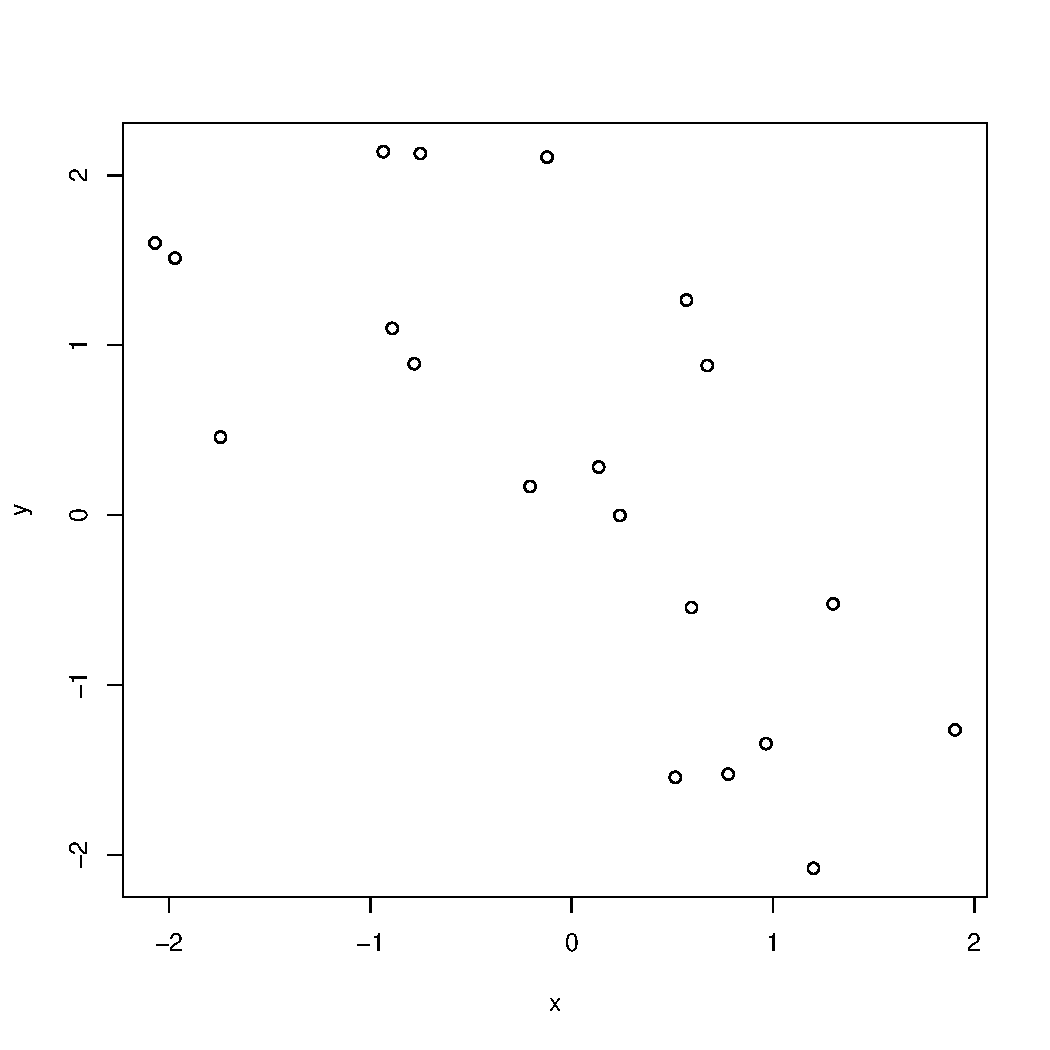
\includegraphics[scale=0.25]{figures/scatter}
  \\
  \tiny 
\end{figure}
\end{frame}
%----------------------------------------------------------------------%
\begin{frame}[fragile]
\frametitle{Direct Sampling}  
\framesubtitle{Example: Linear regression}
\begin{itemize}
\item Step 1: we generate S draws from the $N\left( m,V \right),\ \left\{ \beta^{i} \right\} 1,\ldots,S$
\item $m = \  - 1.07$
\item $V = \ 0.0510$
\end{itemize}

\begin{figure}[H] \centering
  \centering
  \caption{Example of draws $\left( \left\{ \beta^{i} \right\}_{1,\ldots,N} \right),\ S = 1,000$}
  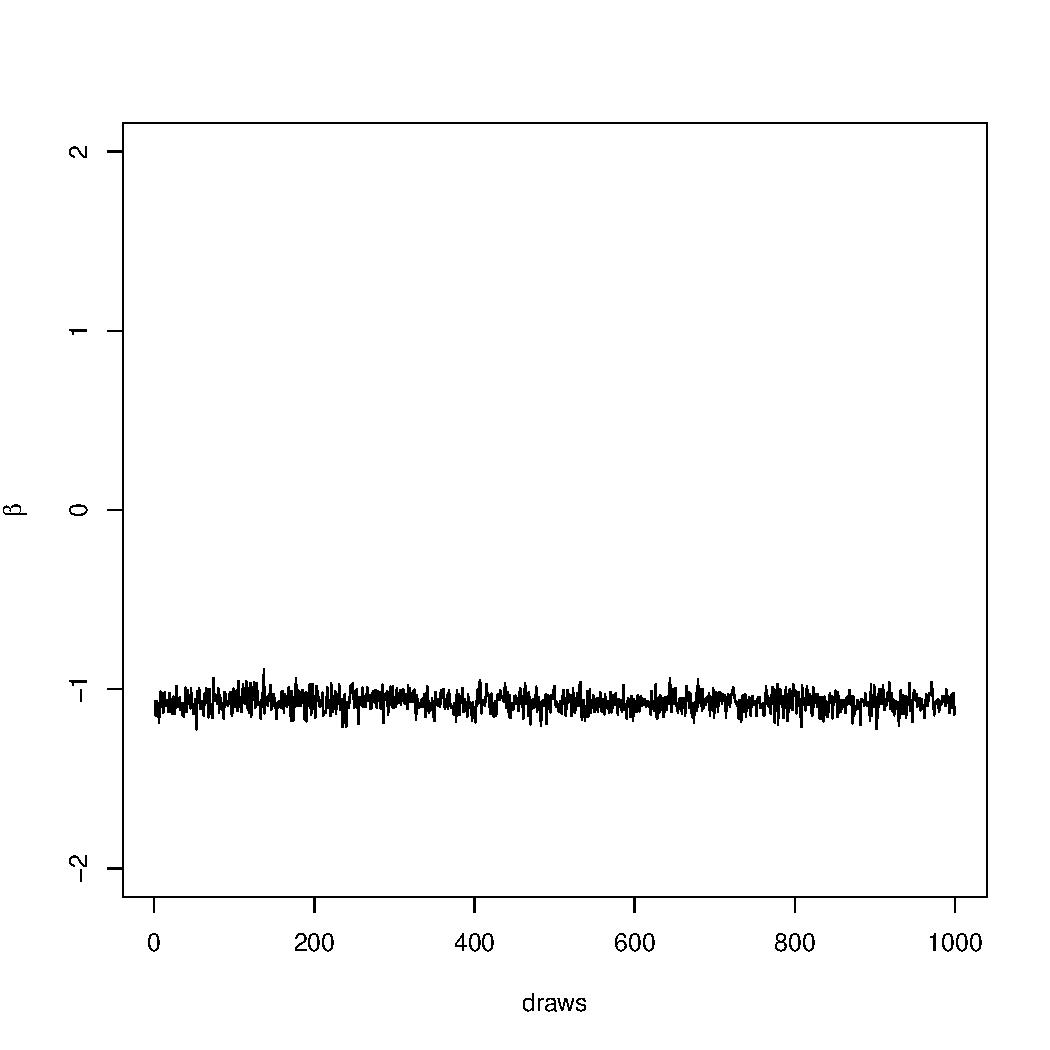
\includegraphics[scale=0.25]{figures/beta}
  \\
  \tiny 
\end{figure}

  
\end{frame}
%----------------------------------------------------------------------%
\begin{frame}[fragile]
\frametitle{Direct Sampling}
\framesubtitle{Example: Linear regression}
\begin{itemize}

\item Step 2: we are interested in posterior moments of $|\beta|$. 
\item Turn draws into $\ \left\{ \left| \beta \right| \right\}_{1,\ldots,S}$
\end{itemize}

\begin{figure}[H] \centering
  \centering
  \caption{Example of draws $\left( \left\{ |\beta^{i}| \right\}_{1,\ldots,S} \right)$}
  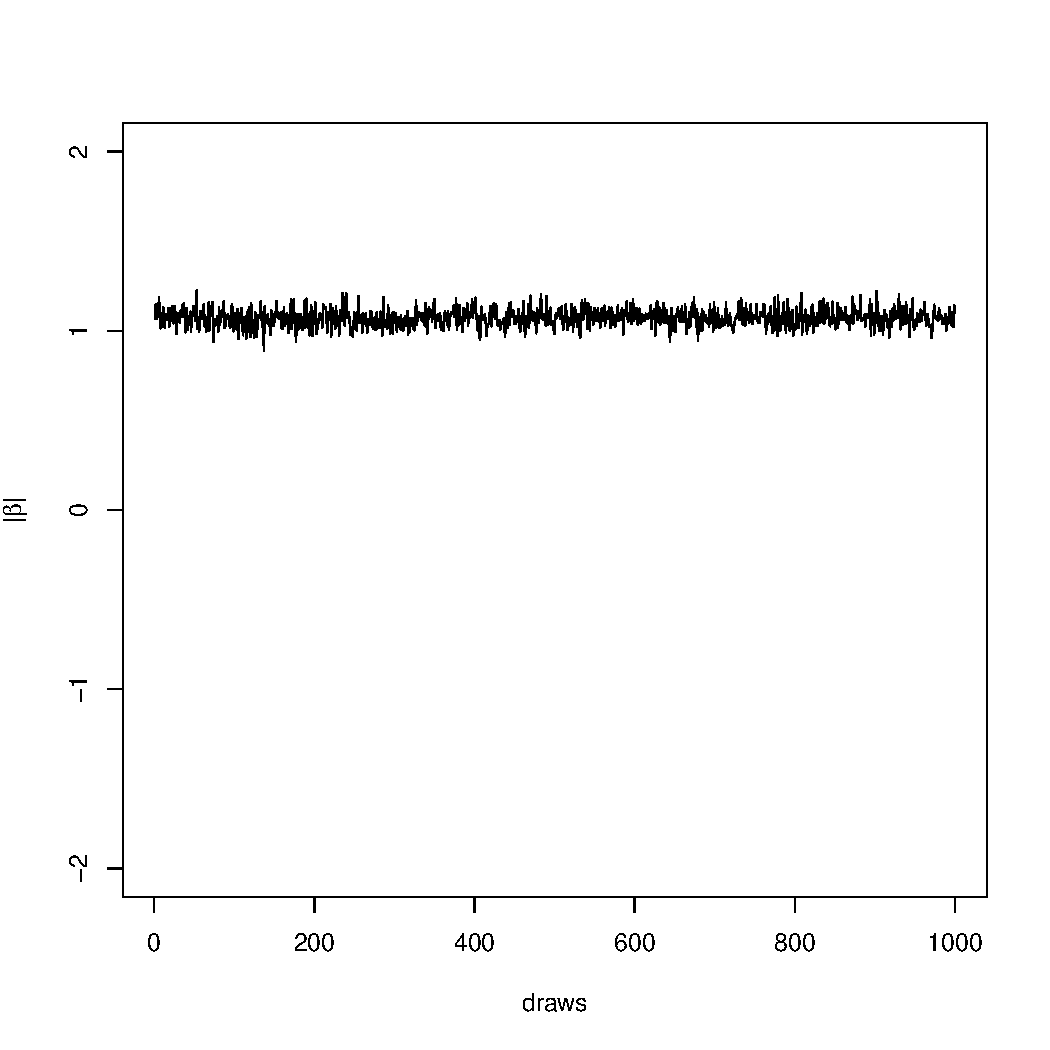
\includegraphics[scale=0.25]{figures/abs}
  \\
  \tiny 
\end{figure}




\end{frame}
%----------------------------------------------------------------------%
\begin{frame}[fragile]
\frametitle{Direct Sampling}  
\framesubtitle{Example: Linear regression}

\begin{itemize}
\item Histogram approximation to $\pi\left( \left| \beta \right|\ |Y \right)$ using $\left\{ \left| \beta^{i} \right| \right\}_{1,\ldots,S}$

  \end{itemize}

\begin{figure}[H] \centering
  \centering
  \caption{Example of draws $\left( \left\{ |\beta^{i}| \right\}_{1,\ldots,S} \right)$}
  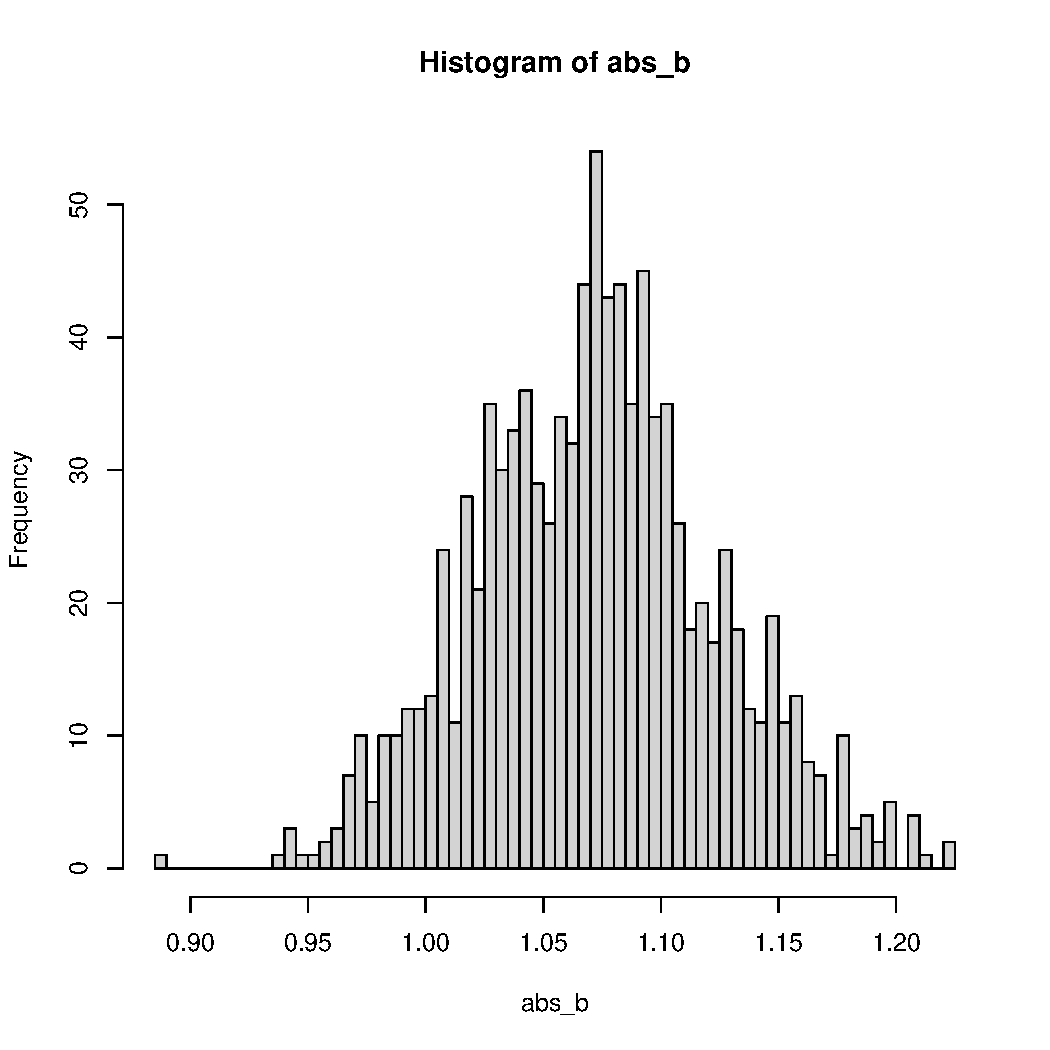
\includegraphics[scale=0.25]{figures/hist}
  \\
  \tiny 
\end{figure}
\end{frame}
%----------------------------------------------------------------------%
\begin{frame}[fragile]
\frametitle{Direct Sampling}  
\framesubtitle{Example: Linear regression}

\begin{itemize}
\item The posterior mean of $\left| \beta \right|$ is approximated by

\begin{align}
E_{Y}^{\beta}\left\lbrack \left| \beta \right| \right\rbrack \approx \frac{1}{S}\ \sum_{i = 1}^{S}{\left| \beta^{i} \right| = 1.0719}
\end{align}

\item The 90\% equal-tail-probability interval is approximated by

\begin{align}
C_{Y} = \left\lbrack q_{l},\ q_{u} \right\rbrack = \lbrack 0.719,\ 1.441\rbrack
\end{align}


\item Where $q_{l}$ and $q_{u}$ such that

\begin{align}
5\% = \ \frac{1}{S}\ \sum_{i = 1}^{S}{1\{\left| \beta \right| < q_{u}\}}
\end{align}
\end{itemize}

\end{frame}
%----------------------------------------------------------------------%
\begin{frame}[fragile]
\frametitle{Direct Sampling}
\framesubtitle{Example: Linear regression}

\begin{itemize}
\item Numerical accuracy of $\frac{1}{S}\ \sum_{i = 1}^{S}{1\left| \beta^{i} \right|}$
\medskip
\item We know that if we generate enough number of $\beta^{i}$, we get an accurate approximation to the posterior moments
\medskip
\item How many draws are enough?
\medskip
\item In other words, "Will I get different answer if I construct the same quantity using different set of draws ${\{\beta}^{i}\}$?
\medskip
\item Is $S = 10$ enough? Or, is $S = 10,000\ $enough?
\end{itemize}
\end{frame}
%----------------------------------------------------------------------%
\begin{frame}[fragile]
\frametitle{Direct Sampling}
\framesubtitle{Example: Linear regression}

\begin{itemize}
\item To see the numerical error I generate 1,000 sets of $\left\{ \beta^{i} \right\}_{i = 1,\ldots,S}$

\item Compute 1,000 of $\frac{1}{S}\ \sum_{i = 1}^{S}\left| \beta^{i} \right|$ to see how variable this Monte Carlo approximation with different $S$

\end{itemize}


  \begin{figure}[H] \centering
  \centering
  \caption{Distribution of $\frac{1}{S}\ \sum_{i = 1}^{S}{\ \left| \beta^{i} \right|}$ over $\left\{ \beta^{i} \right\}_{i = 1,\ldots,S}$}
  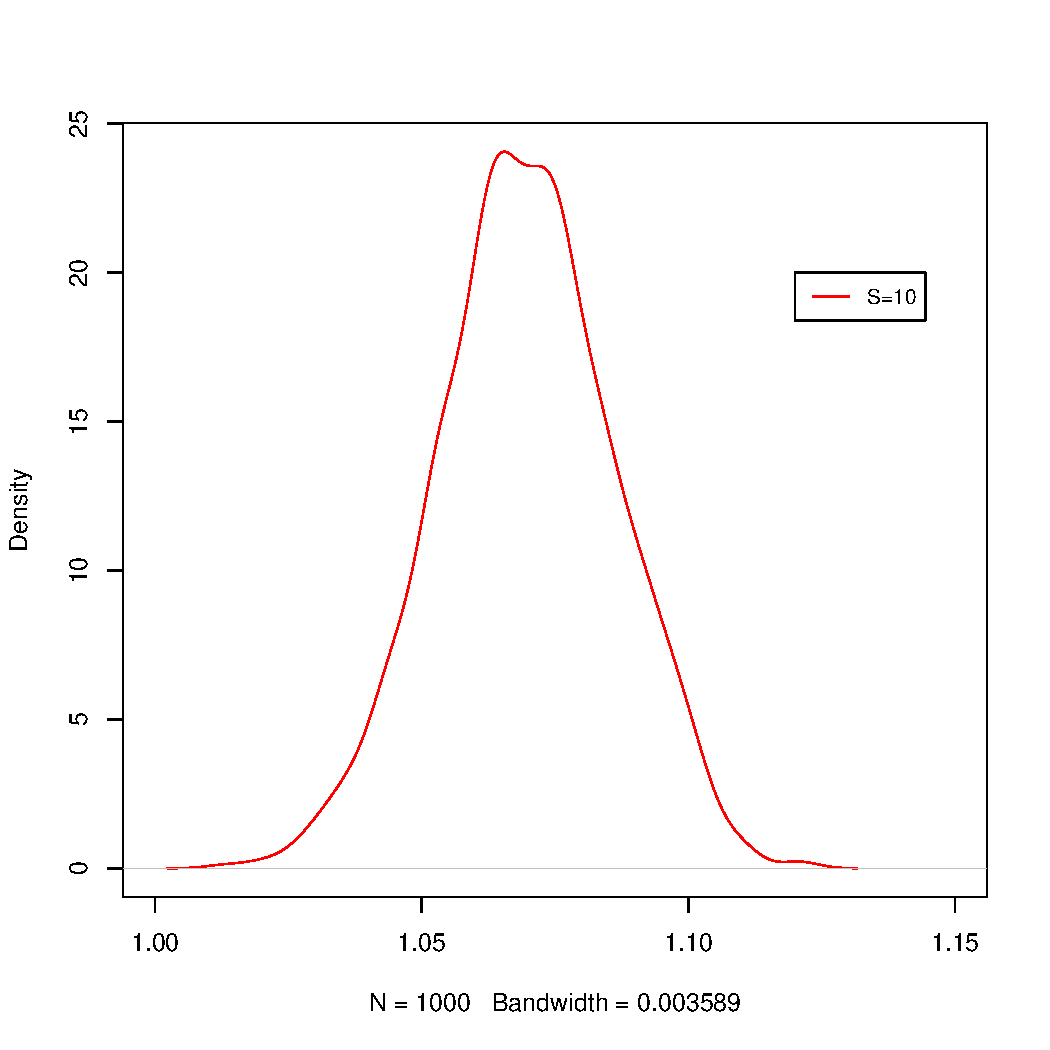
\includegraphics[scale=0.2]{figures/n10}
  \\
  \tiny 
  $\text{SD\ }\frac{1}{S}\ \sum_{i = 1}^{S}{\ \left| \beta^{i} \right|} = 0.688$
\end{figure}




\end{frame}
%----------------------------------------------------------------------%
\begin{frame}[fragile]
\frametitle{Direct Sampling}
\framesubtitle{Example: Linear regression}

\begin{itemize}
\item To see the numerical error I generate 1,000 sets of $\left\{ \beta^{i} \right\}_{i = 1,\ldots,S}$

\item Compute 1,000 of $\frac{1}{S}\ \sum_{i = 1}^{S}\left| \beta^{i} \right|$ to see how variable this Monte Carlo approximation with different $S$

\end{itemize}




  \begin{figure}[H] \centering
  \centering
  \caption{Distribution of $\frac{1}{S}\ \sum_{i = 1}^{S}{\ \left| \beta^{i} \right|}$ over $\left\{ \beta^{i} \right\}_{i = 1,\ldots,S}$}
  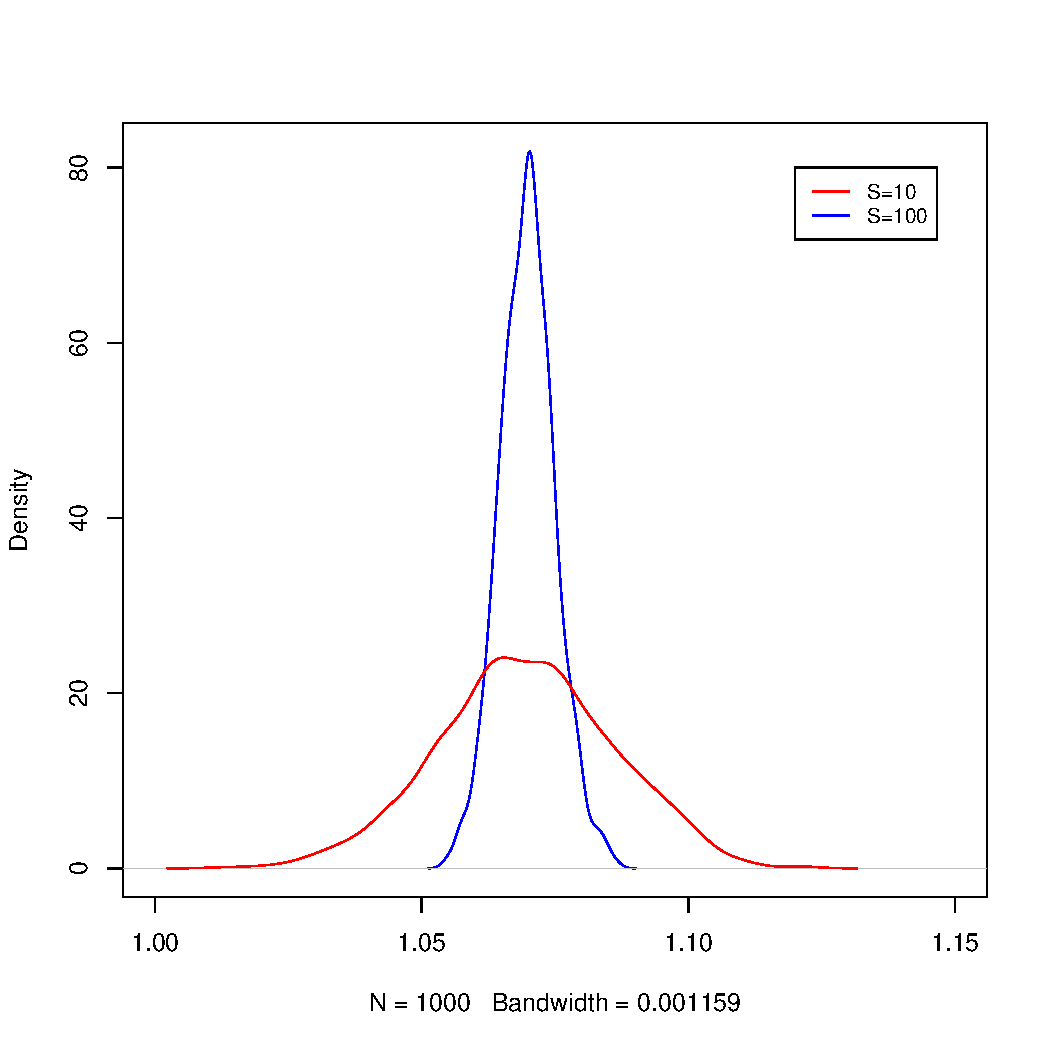
\includegraphics[scale=0.2]{figures/n100}
  \\
  \tiny 
  $$\text{SD\ }\frac{1}{S}\ \sum_{i = 1}^{S}{\ \left| \beta^{i} \right|} = 0.022$$
\end{figure}  




\end{frame}
%----------------------------------------------------------------------%
\begin{frame}[fragile]
\frametitle{Direct Sampling}
\framesubtitle{Example: Linear regression}

\begin{itemize}
\item To see the numerical error I generate 1,000 sets of $\left\{ \beta^{i} \right\}_{i = 1,\ldots,S}$

\item Compute 1,000 of $\frac{1}{S}\ \sum_{i = 1}^{S}\left| \beta^{i} \right|$ to see how variable this Monte Carlo approximation with different $S$

\end{itemize}


  

  \begin{figure}[H] \centering
  \centering
  \caption{Distribution of $\frac{1}{S}\ \sum_{i = 1}^{S}{\ \left| \beta^{i} \right|}$ over $\left\{ \beta^{i} \right\}_{i = 1,\ldots,S}$}
  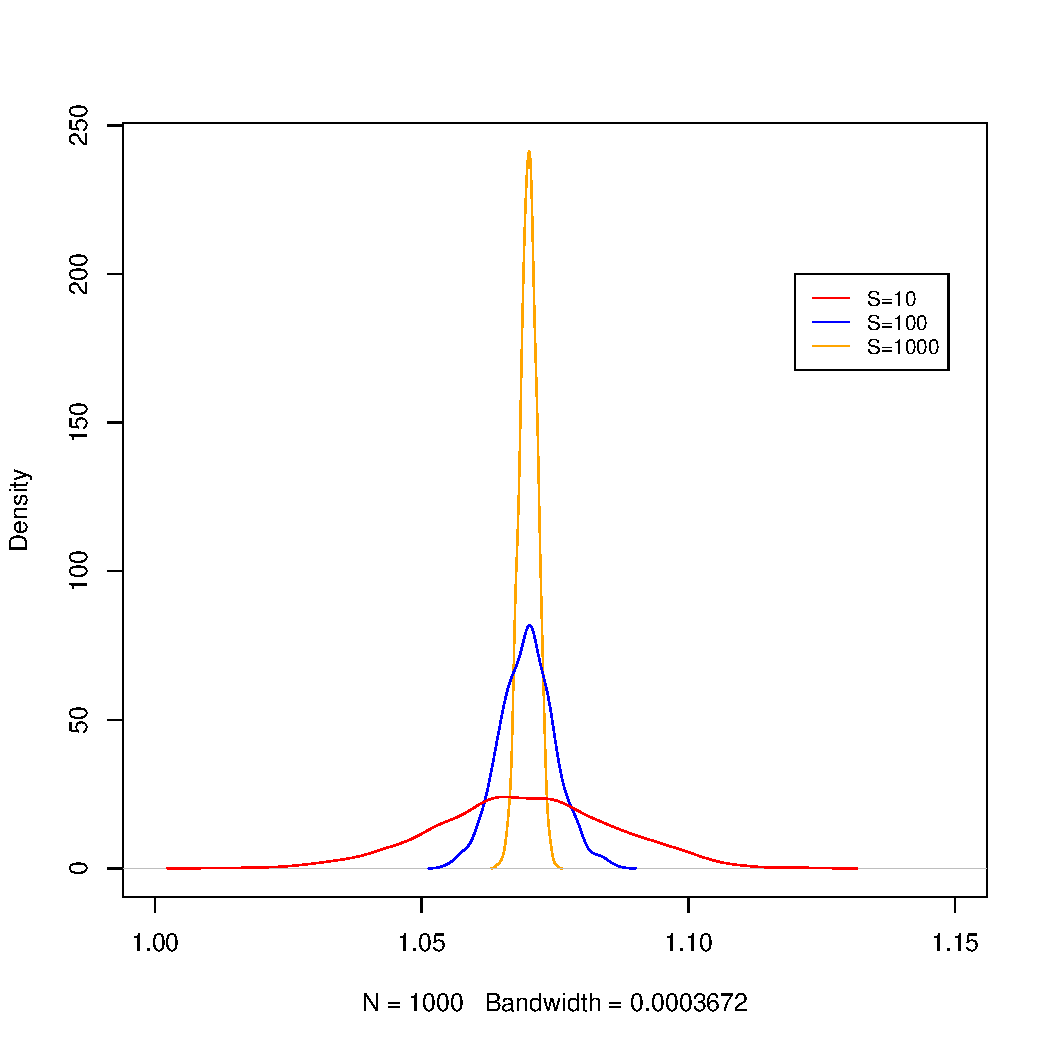
\includegraphics[scale=0.2]{figures/n1000}
  \\
  \tiny 
  $$\text{SD\ }\frac{1}{S}\ \sum_{i = 1}^{S}{\ \left| \beta^{i} \right|} = 0.0074$$
\end{figure}  




\end{frame}
%----------------------------------------------------------------------%
\begin{frame}[fragile]
\frametitle{Direct Sampling}
\framesubtitle{Example: Linear regression}

\begin{itemize}
\item To see the numerical error I generate 1,000 sets of $\left\{ \beta^{i} \right\}_{i = 1,\ldots,S}$

\item Compute 1,000 of $\frac{1}{S}\ \sum_{i = 1}^{S}\left| \beta^{i} \right|$ to see how variable this Monte Carlo approximation with different $S$

\end{itemize}



  \begin{figure}[H] \centering
  \centering
  \caption{Distribution of $\frac{1}{S}\ \sum_{i = 1}^{S}{\ \left| \beta^{i} \right|}$ over $\left\{ \beta^{i} \right\}_{i = 1,\ldots,S}$}
  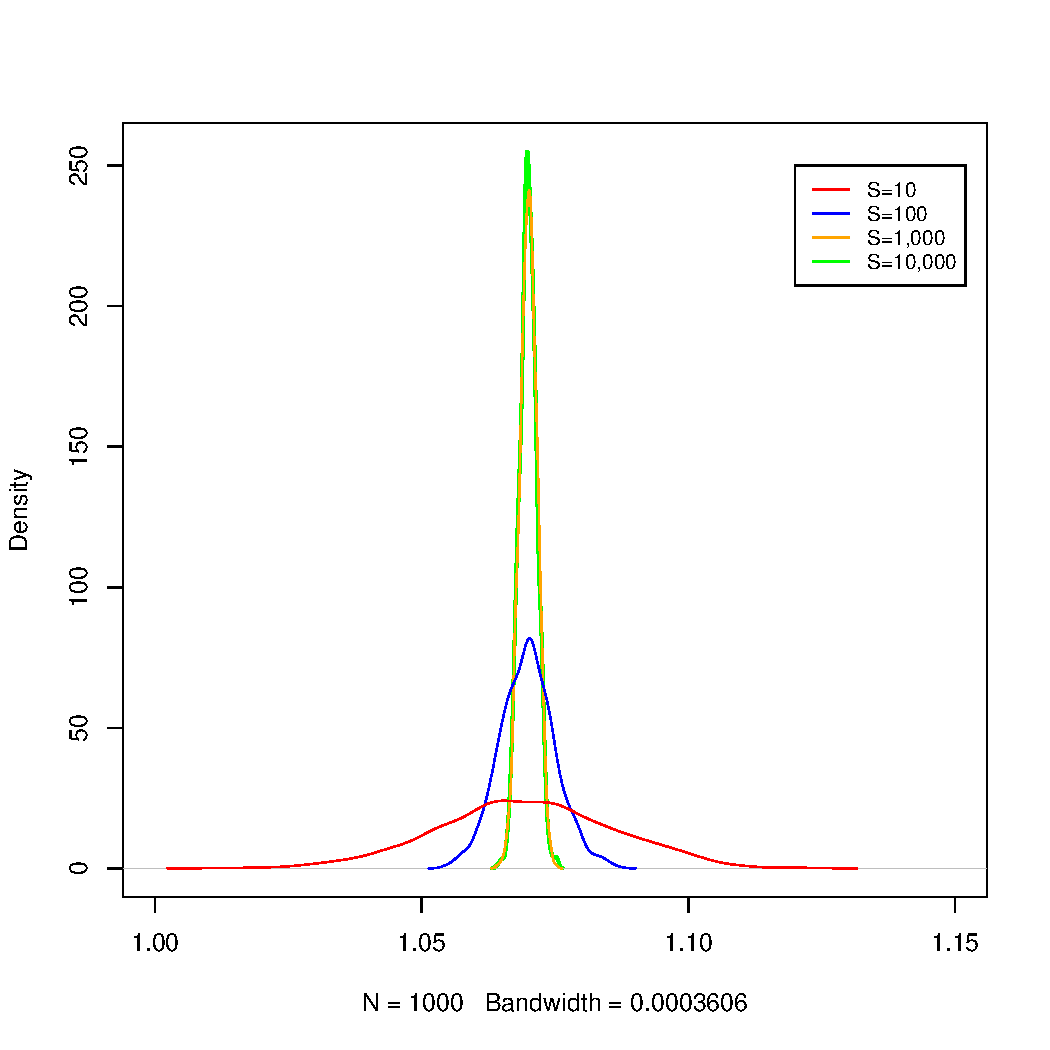
\includegraphics[scale=0.2]{figures/n10000}
  \\
  \tiny 
  $$\text{SD\ }\frac{1}{S}\ \sum_{i = 1}^{S}{\ \left| \beta^{i} \right|} = 0.0023$$
\end{figure}  




 \end{frame}
%----------------------------------------------------------------------%
\begin{frame}[fragile]
\frametitle{Direct Sampling} 
\framesubtitle{Example: Linear regression}

\begin{itemize}

\item What do we try to capture in this exercise?
\medskip
\item We try to mimic the distribution of Monte Carlo approximation offered by
\medskip
\begin{align}
\sqrt{S}\ \left( \frac{1}{S}\ \sum_{i = 1}^{N}{h\left( \beta^{i} \right) - \ \int_{}^{}{h\left( \beta \right)\pi\left( \beta \middle| Y \right) d\beta}} \right)\  \rightarrow_{d}\ N(0,V_{\pi})
\end{align}
\medskip
\item All variation in this Monte Carlo approximation is due to numerical "simulation".
\medskip
\item Throughout this example, we fix $Y_{1:N},\ X_{1:N}$ (not a sampling variation).
\end{itemize}
\end{frame}

%----------------------------------------------------------------------%
\section{Recap}
%----------------------------------------------------------------------%
\begin{frame}[fragile]
\frametitle{Recap} 

\begin{itemize}
\item If you know how to generate $\text{i.i.d}$ draws from the posterior distribution of $\beta$,

\item You also can posterior moments of $h(\beta)$ by simple average:
\begin{align}
\int_{}^{}{\text{h\ }\left( \beta \right)p\left( \beta \middle| Y \right)d\beta}\  \approx \ \frac{1}{S}\ \sum_{i = 1}^{S}{h (\beta^{i})}
\end{align}
\item  SLLN guarantees this Monte Carlo average to the right limit:

\begin{align}
\frac{1}{S} \sum_{i = 1}^{S}{h\left( \beta^{i} \right) \rightarrow_{\text{a.s}} \int_{}^{} h\left( \beta \right)\pi\left( \beta | Y \right)d\beta }
\end{align}

\item CLT tells you that the Monte Carlo average always has a numerical error:

\begin{align}
\sqrt{S} \left( \frac{1}{S} \sum_{i = 1}^{N} h \left( \beta^{i} \right) - \int_{}^{}{h\left( \beta \right)\pi\left( \beta| Y \right)d\beta } \right)  \rightarrow_{d}\ N\ (0,V_{\pi}) 
\end{align}
\item  It is important to check how good is your numerical approximation
\end{itemize}
\end{frame}


%----------------------------------------------------------------------%
\begin{frame}
\frametitle{Review \& Next Steps}
  
  \begin{itemize} 
    
    
    \item Direct Sampler
  \bigskip  

  
  \item  {\bf Next Class:} Gibbs Sampler

  
  
  \end{itemize}


\end{frame}
%----------------------------------------------------------------------%

\section{Further Readings}
%----------------------------------------------------------------------%
\begin{frame}
\frametitle{Further Readings}

\begin{itemize}
  \item Casella, G., \& Berger, R. L. (2002). Statistical inference (Vol. 2, pp. 337-472). Pacific Grove, CA: Duxbury. Chapter 7
  \medskip
  \item Hoff, P. D. (2009). A first course in Bayesian statistical methods (Vol. 580). New York: Springer.
  \medskip
  
  
  
\end{itemize}

\end{frame}

%----------------------------------------------------------------------%
%----------------------------------------------------------------------%

\end{document}

%----------------------------------------------------------------------%
%----------------------------------------------------------------------%

